\section{Future Directions for Inclusive Unpolarized EMC Effect Measurements}

With the observation that the EMC Effect appears to be driven by the local nuclear environment
and the apparent connection between the EMC Effect and short range correlations, it is worth examining what
further studies with inclusive electron scattering can shed light on the origin of the EMC Effect.

One clear avenue of exploration is to make EMC Effect measurements from additional light to medium-light
nuclei where ab-initio nuclear structure calculations are feasible and interesting nuclear cluster
structures may manifest.

Additionally, one can leverage the fact that SRCs are dominated by neutron-proton pairs to further explore
the robustness of the EMC-SRC correlation by measuring the EMC Effect for a range of nuclei with
different neutron to proton ($N/P$) ratio at fixed $A$, and for a range of $A$ at fixed $N/P$.

Both of the above will be accomplished by JLab experiment E12-10-008~\cite{12gev_emc} in combination
with E12-06-105~\cite{12gev_xgt1}. E12-10-008 will measure the EMC Effect for a wide range of nuclei,
aimed at elucidating the EMC-SRC connection, providing first measurements for a variety of light nuclei,
and exploring in-medium $n/p$ ratios via measurements of $A$ and $A\pm1$ nuclei.  E12-06-105 will make
measurements at $x>1$ in the two-nucleon correlation region for the same nuclei as well as make additional
measurements in search of possible three-nucleon correlations. Figure~\ref{fig:np_ratios} shows the $N/P$
ratio vs. $A$ for the nuclear targets that will be used for both experiments.

\begin{figure}[htb]
  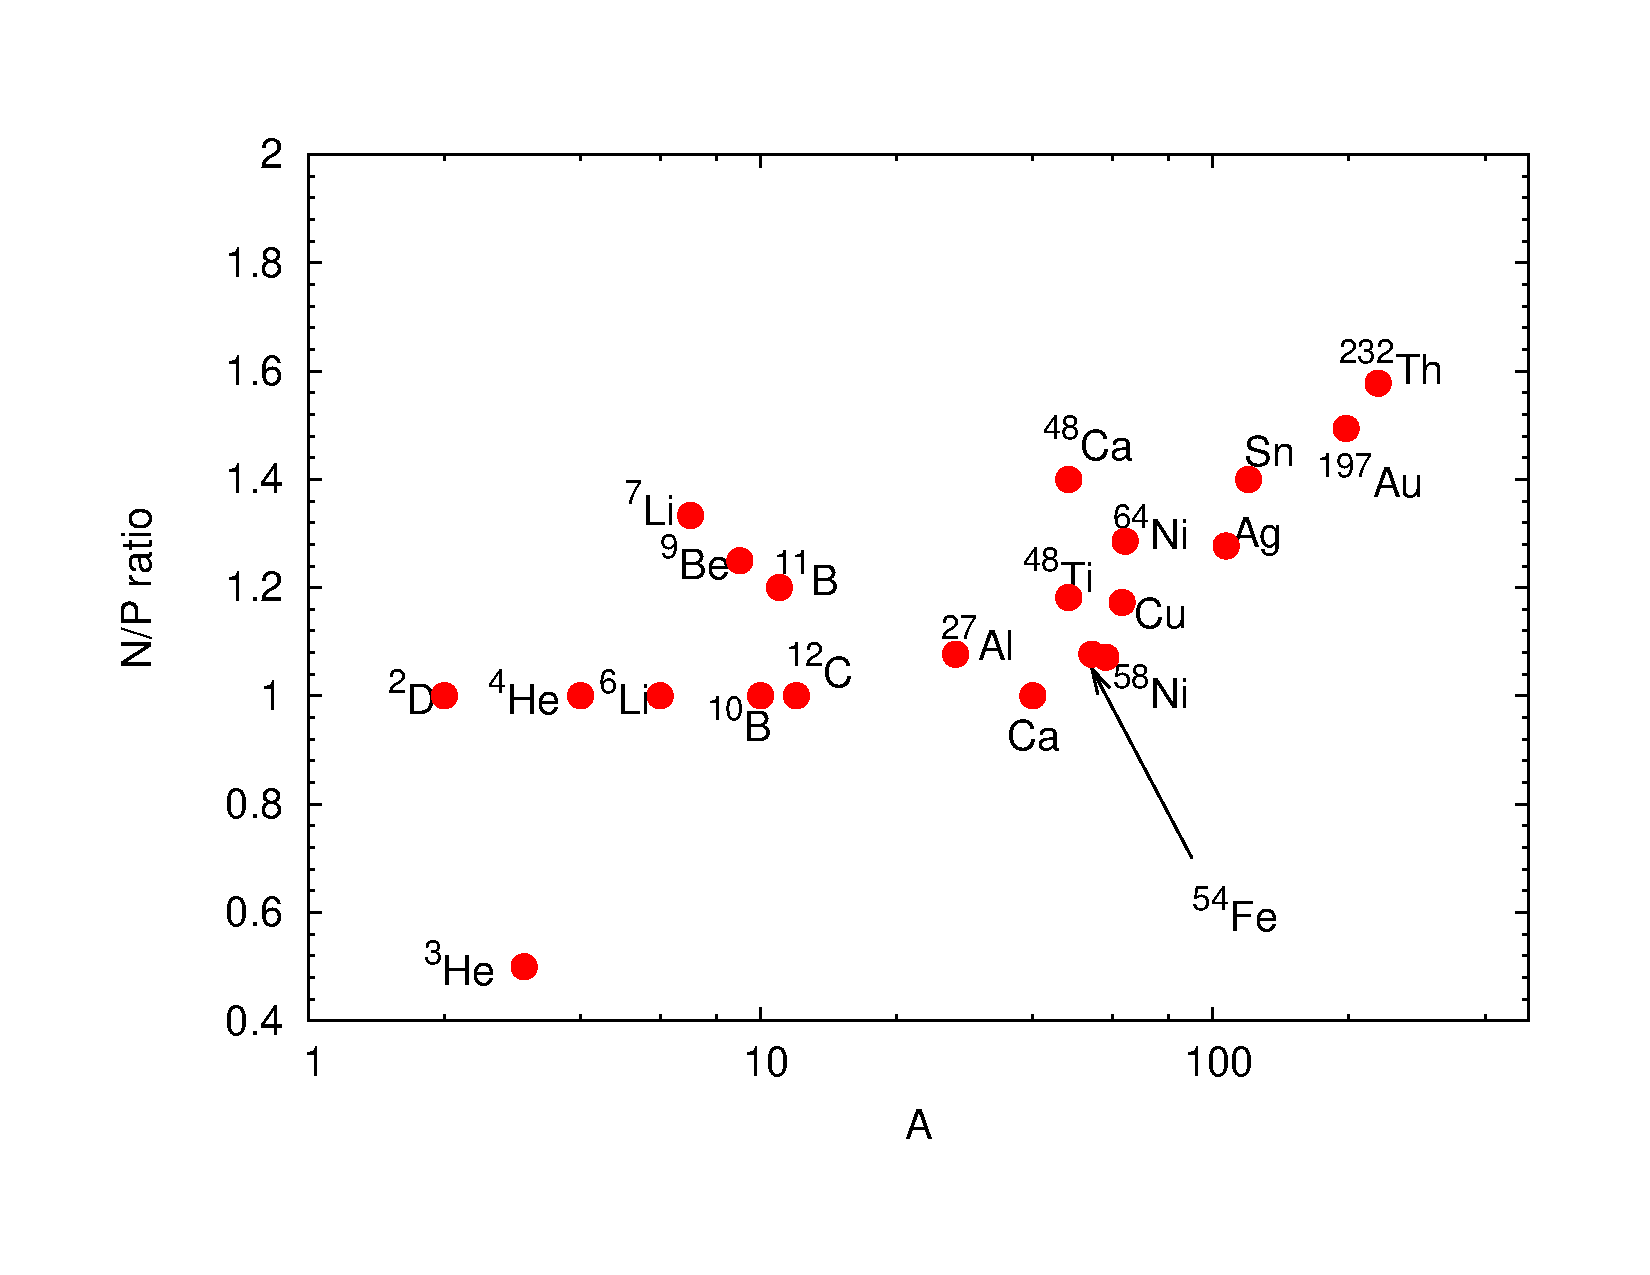
\includegraphics[width=0.5\textwidth]{plots/np_ratios_2017.pdf}
  \caption{$N/P$ ratio vs. $A$ for nuclei that will be measured by JLab experiments E12-10-008 (EMC Effect)
    and E12-06-105 ($x>1$) to further elucidate the apparent link between the EMC Effect and short range
    correlations. Figure courtesy of N. Fomin.}
  \label{fig:np_ratios}
\end{figure}